\chapter{网格自适应性}

\section{网格自适应加密放粗}

网格自适应可以分为局部加密放粗和全局加密放粗,局部和全局的区别关键在于对初始网格的处理,局部网格剖分是对初始网格的修改,而全局网格剖分会重新生成新的网格。
局部加密放粗可以分为按顶点加密放粗和按单元加密放粗,全局加密放粗可以采用quadtree-octree(四叉树/八叉树)、advancing-front(前沿推进)和Delaunay类型的。
图\ref{fig:2-1}中用两个简单的例子说明按顶点加密放粗和按单元加密放粗,左上分图里红点为顶点,围绕该顶点有两条边,对两条边取中点得到两个新点,并和原有顶点相连,进行了细分,
左下分图里两个红点代表两个单元,将两个单元相邻边取中点,和边对面的顶点相连,分别将两个单元进行了细分得到了四个单元,并且保持协调性。全局加密放粗计算量大于局部,此外还有
hierarchic methods(继承方法)、多重网格、非协调和重叠方法,还需要考虑各向异性。

\begin{figure}[!htbp]
  \centering
  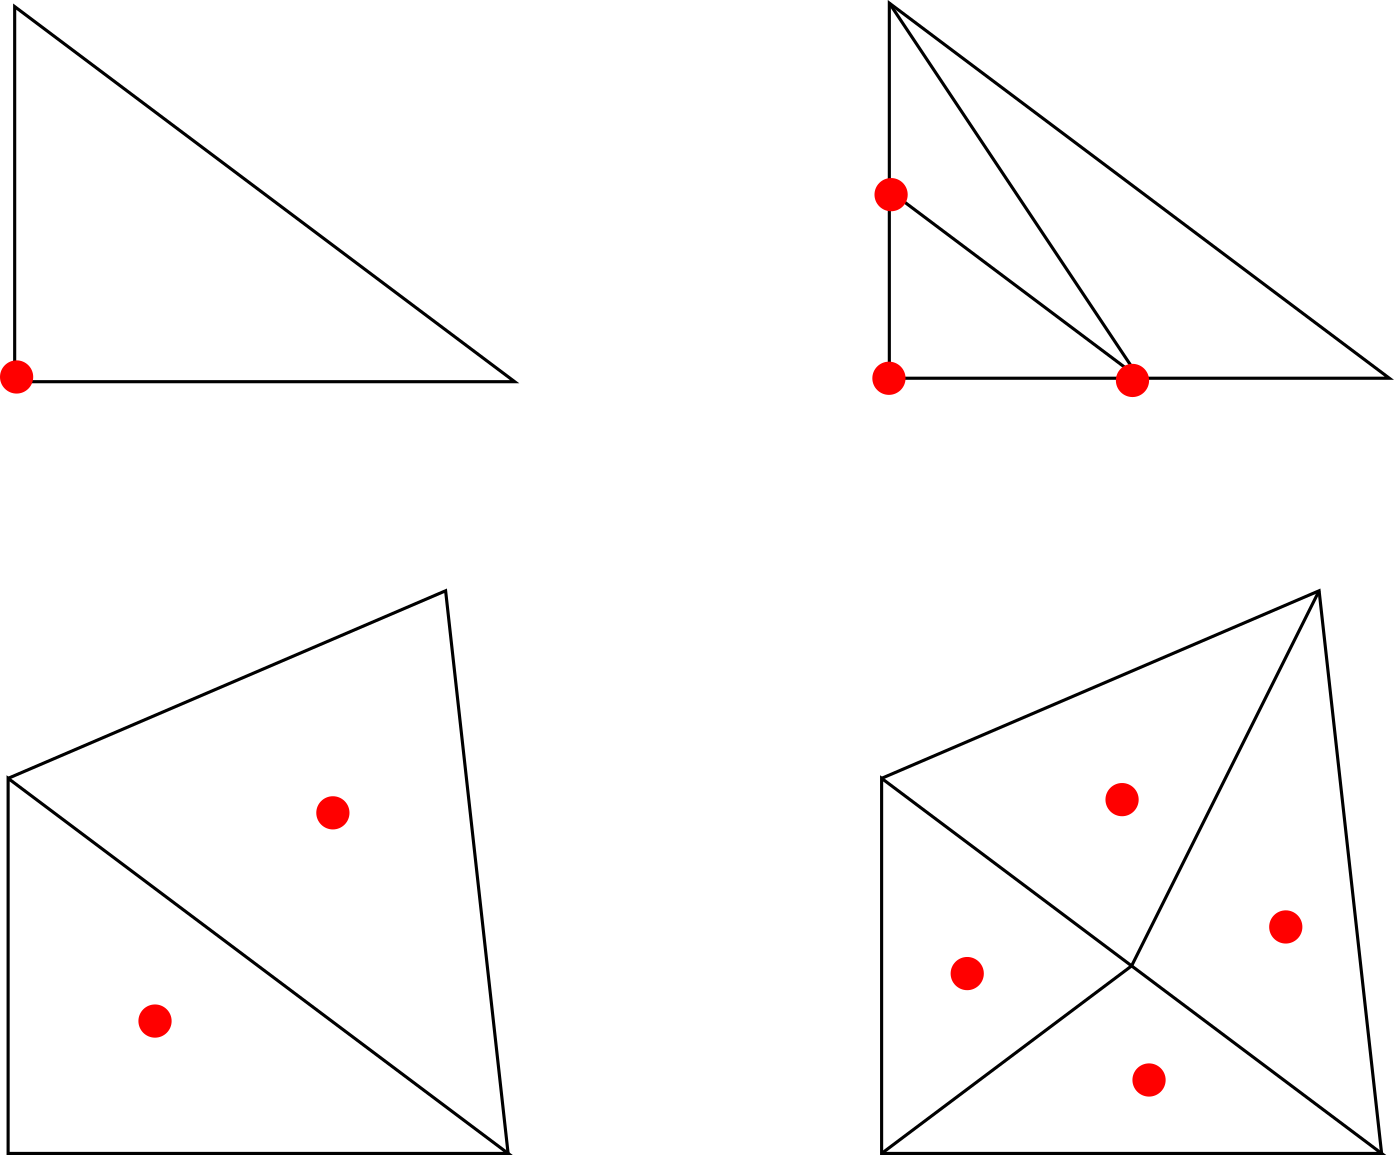
\includegraphics[height=5cm]{fig/2/1.png}
  \caption{按定点加密放粗和按单元加密放粗}
  \label{fig:2-1}
\end{figure}

以Tetgen为例测试局部加密放粗。第一个例子是通过插入点进行加密,第二个例子是通过设置单元大小进行加密,第三个例子是通过设置顶点网格密度进行加密。第一个例子通过.off格式文件读入
多面体,同时通过.node格式文件读入插入点,需要在操作命令序列中设置i命令。第二个例子需要读入网格文件,包括单元、面、边、点,同时通过.vol格式文件读入单元大小,需要注意的是操作命令序列中需要先设置r命令再设置a命令,设置r才会读入.vol文件,设置a会按照单元大小加密。第三个例子通过.poly格式文件读入多面体,同时通过.mtr格式文件读入顶点网格密度,需要在操作命令序列中设置m命令。

\subsection{插点自适应加密}

\begin{figure}[!htbp]
  \centering
  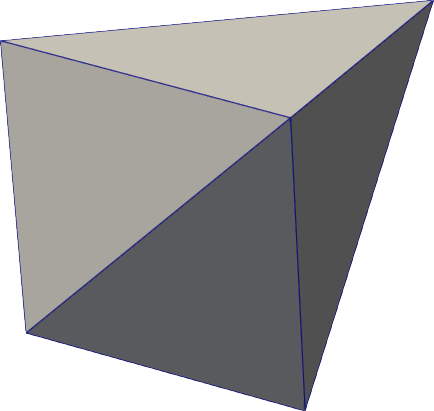
\includegraphics[height=3cm]{fig/2/2.png}
  \caption{例一:原始网格}
  \label{fig:2-1}
\end{figure}

\begin{figure}[!htbp]
  \centering
  
\includegraphics[height=3cm]{fig/2/3.png}
  \caption{例一:插入1个点进行加密}
  \label{fig:2-1}
\end{figure}

\begin{figure}[!htbp]
  \centering
  
\includegraphics[height=3cm]{fig/2/4.png}
  \caption{例一:插入7个点进行加密}
  \label{fig:2-1}
\end{figure}

\begin{figure}[!htbp]
  \centering
  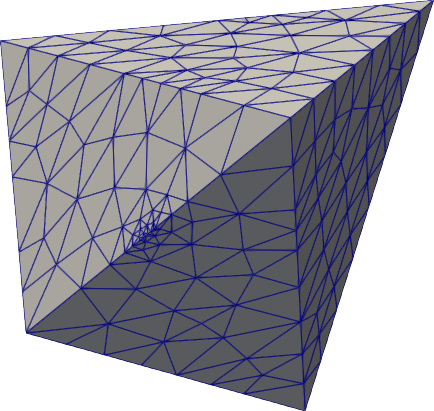
\includegraphics[height=3cm]{fig/2/5.png}
  \caption{例一:原始网格一致加密后(pka0.001i),插入7个点再加密}
  \label{fig:2-1}
\end{figure}

\begin{figure}[!htbp]
  \centering
  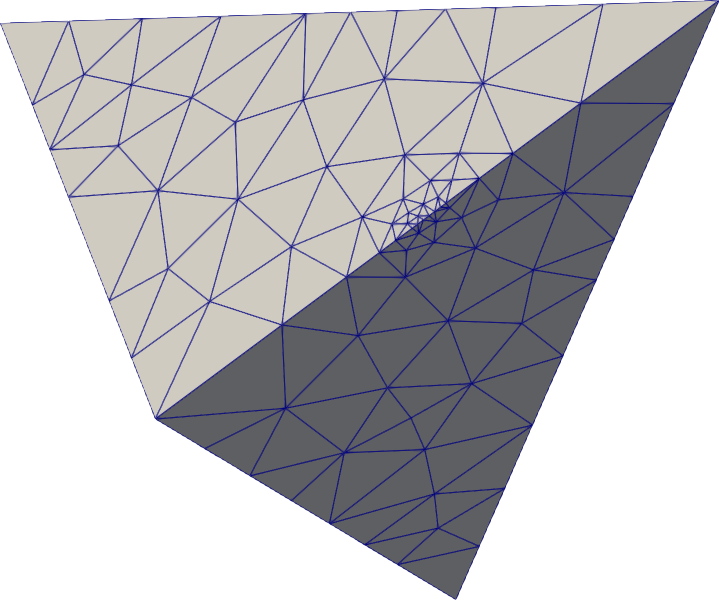
\includegraphics[height=3cm]{fig/2/6.png}
  \caption{例一:原始网格一致加密后(pka0.001i),插入7个点再加密}
  \label{fig:2-1}
\end{figure}

\begin{figure}[!htbp]
  \centering
  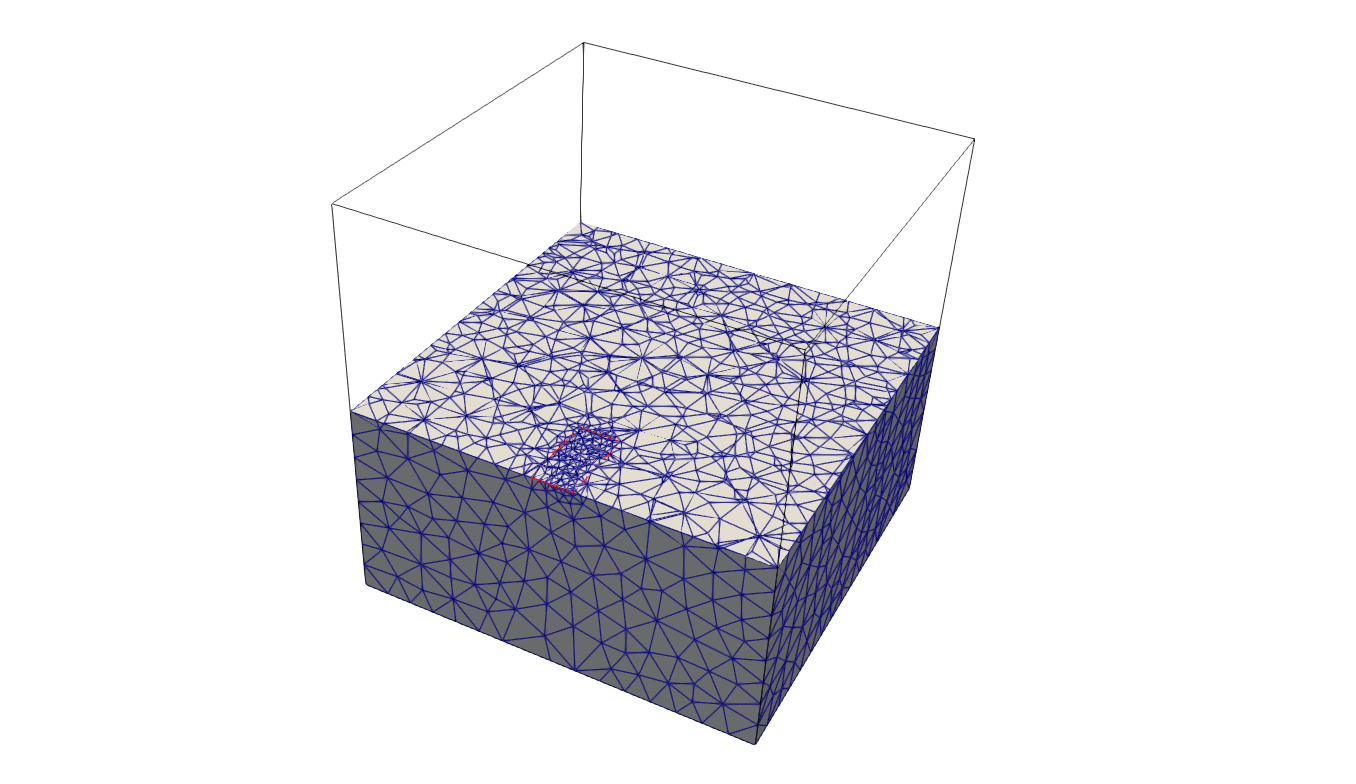
\includegraphics[height=3cm]{fig/2/16.png}
  \caption{向指定位置插入点进行加密}
  \label{fig:2-1}
\end{figure}

\begin{figure}[!htbp]
  \centering
  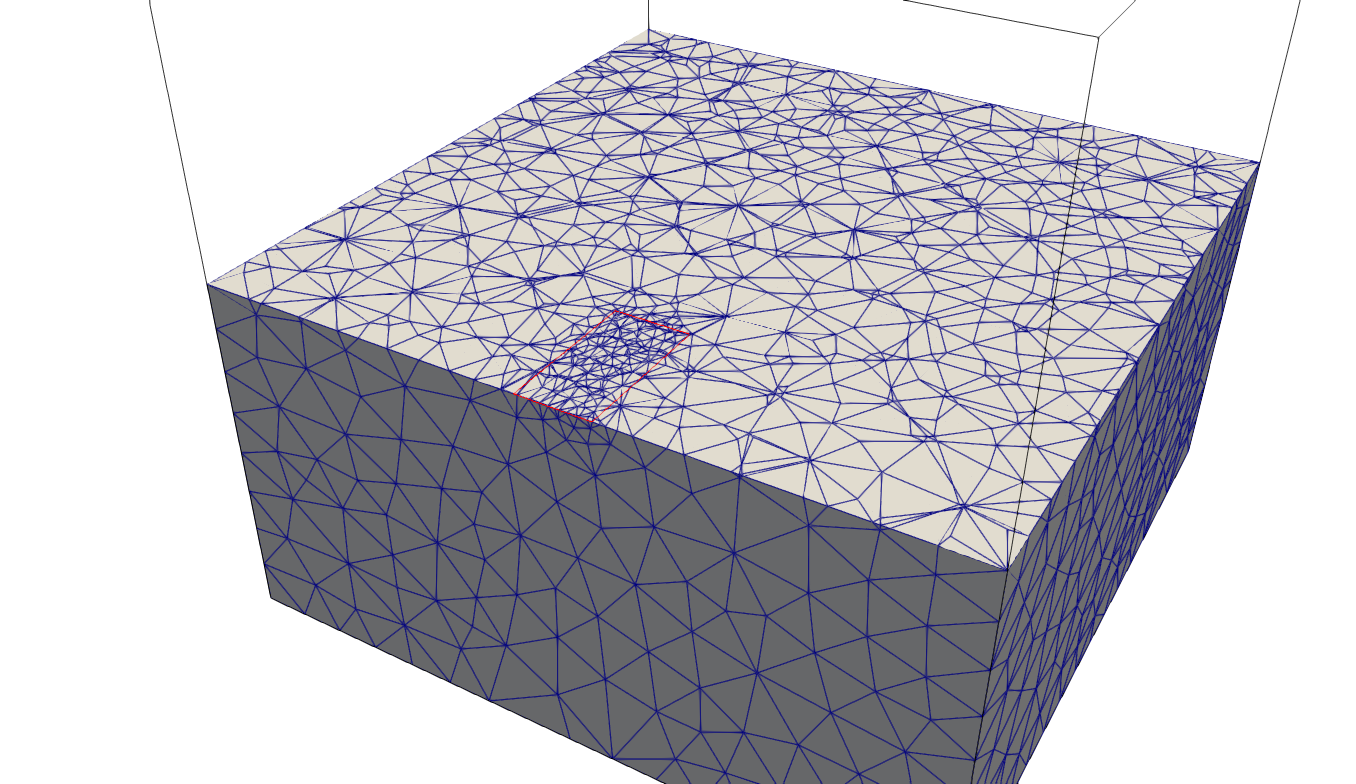
\includegraphics[height=3cm]{fig/2/17.png}
  \caption{向指定位置插入点进行加密}
  \label{fig:2-1}
\end{figure}

\newpage
\subsection{按单元大小自适应加密}\label{se:2.1.2}

\begin{figure}[!htbp]
  \centering
  
\includegraphics[height=3cm]{fig/2/7.png}
  \caption{例二:原始网格,有三个单元}
  \label{fig:2-1}
\end{figure}

\begin{figure}[!htbp]
  \centering
  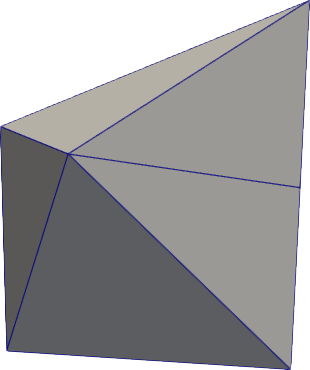
\includegraphics[height=3cm]{fig/2/8.png}
  \caption{例二:将第三个单元大小设置为0.1}
  \label{fig:2-1}
\end{figure}

\begin{figure}[!htbp]
  \centering
  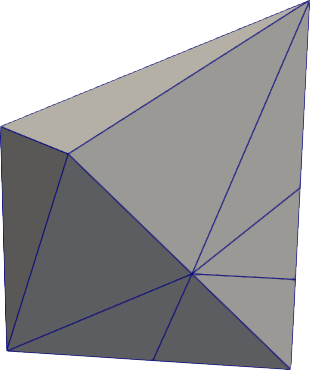
\includegraphics[height=3cm]{fig/2/9.png}
  \caption{例二:将第三个单元大小设置为0.01}
  \label{fig:2-1}
\end{figure}

\begin{figure}[!htbp]
  \centering
  
\includegraphics[height=3cm]{fig/2/10.png}
  \caption{例二:将第三个单元大小设置为0.001}
  \label{fig:2-1}
\end{figure}

\begin{figure}[!htbp]
  \centering
  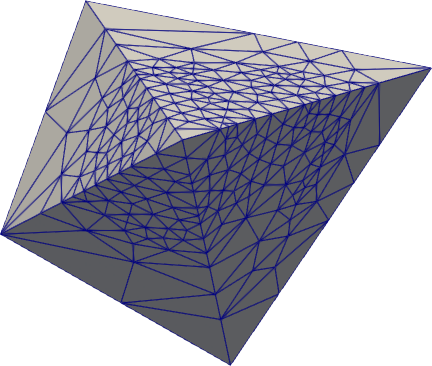
\includegraphics[height=3cm]{fig/2/11.png}
  \caption{例二:将第三个单元大小设置为0.0001}
  \label{fig:2-1}
\end{figure}

\newpage
\subsection{按顶点密度自适应加密}

\begin{figure}[!htbp]
  \centering
  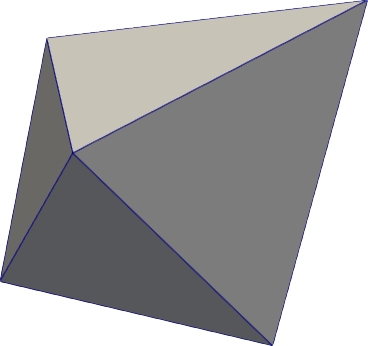
\includegraphics[height=3cm]{fig/2/12.png}
  \caption{例三:原始网格,一共五个顶点}
  \label{fig:2-1}
\end{figure}

\begin{figure}[!htbp]
  \centering
  
\includegraphics[height=3cm]{fig/2/13.png}
  \caption{例三:将所有顶点网格密度设置为0.25}
  \label{fig:2-1}
\end{figure}

\begin{figure}[!htbp]
  \centering
  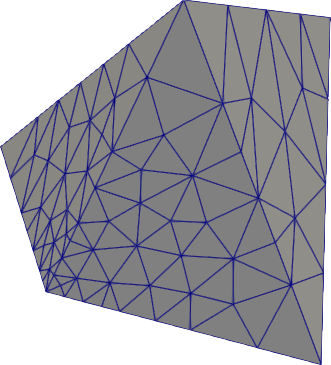
\includegraphics[height=3cm]{fig/2/14.png}
  \caption{例三:将第一个顶点网格密度设置为0.05}
  \label{fig:2-1}
\end{figure}

\begin{figure}[!htbp]
  \centering
  
\includegraphics[height=3cm]{fig/2/15.png}
  \caption{例三:将第一个顶点网格密度设置为0.01}
  \label{fig:2-1}
\end{figure}

\subsection{删点自适应放粗}

以上是网格加密,再看通过删点对网格进行放粗。采用命令序列krR,r命令可以读取网格,R命令删除.node文件中标识为0的点。
\begin{figure}[!htbp]
  \centering
  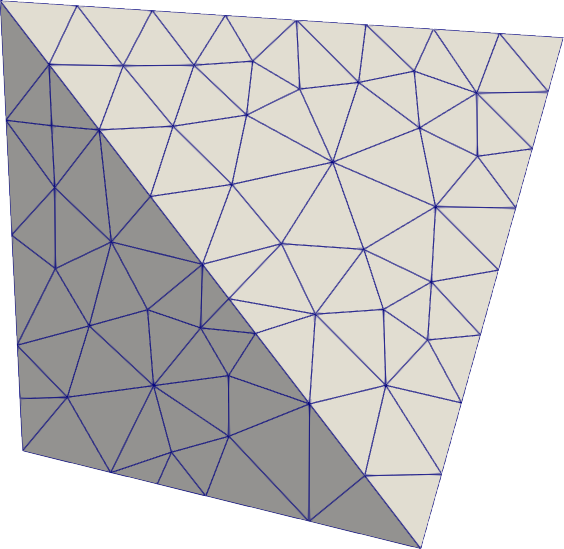
\includegraphics[height=3cm]{fig/2/18.png}
  \caption{原始网格,tetgen命令序列为kr}
  \label{fig:2-1}
\end{figure}

\begin{figure}[!htbp]
  \centering
  
\includegraphics[height=3cm]{fig/2/19.png}
  \caption{删除点放粗后的网格,tetgen命令序列为krR}
  \label{fig:2-1}
\end{figure}


\section{层网格自适应加密放粗}

层网格自适应加密放粗可以采用两种方法,需要考虑到材料增加过程,在变化较大区域按照逐层考虑,在变化较小区域将一定层数进行合并。一种是按照常规网格加密,首先对整个区域逐层进行粗网格剖分,其次将一定层数进行合并,生成更粗的网格,这样获取两套粗网格,然后根据带约束德洛内网格剖分的边界约束,可以将逐层部分和层合并部分根据生死单元激活进行组合,然后设置逐层部分需要加密的单元以及加密参数,对网格进行加密。例如在\ref{se:2.1.2}中,读入网格,读入单元加密大小,进行加密。

\begin{figure}[!htbp]
  \centering
  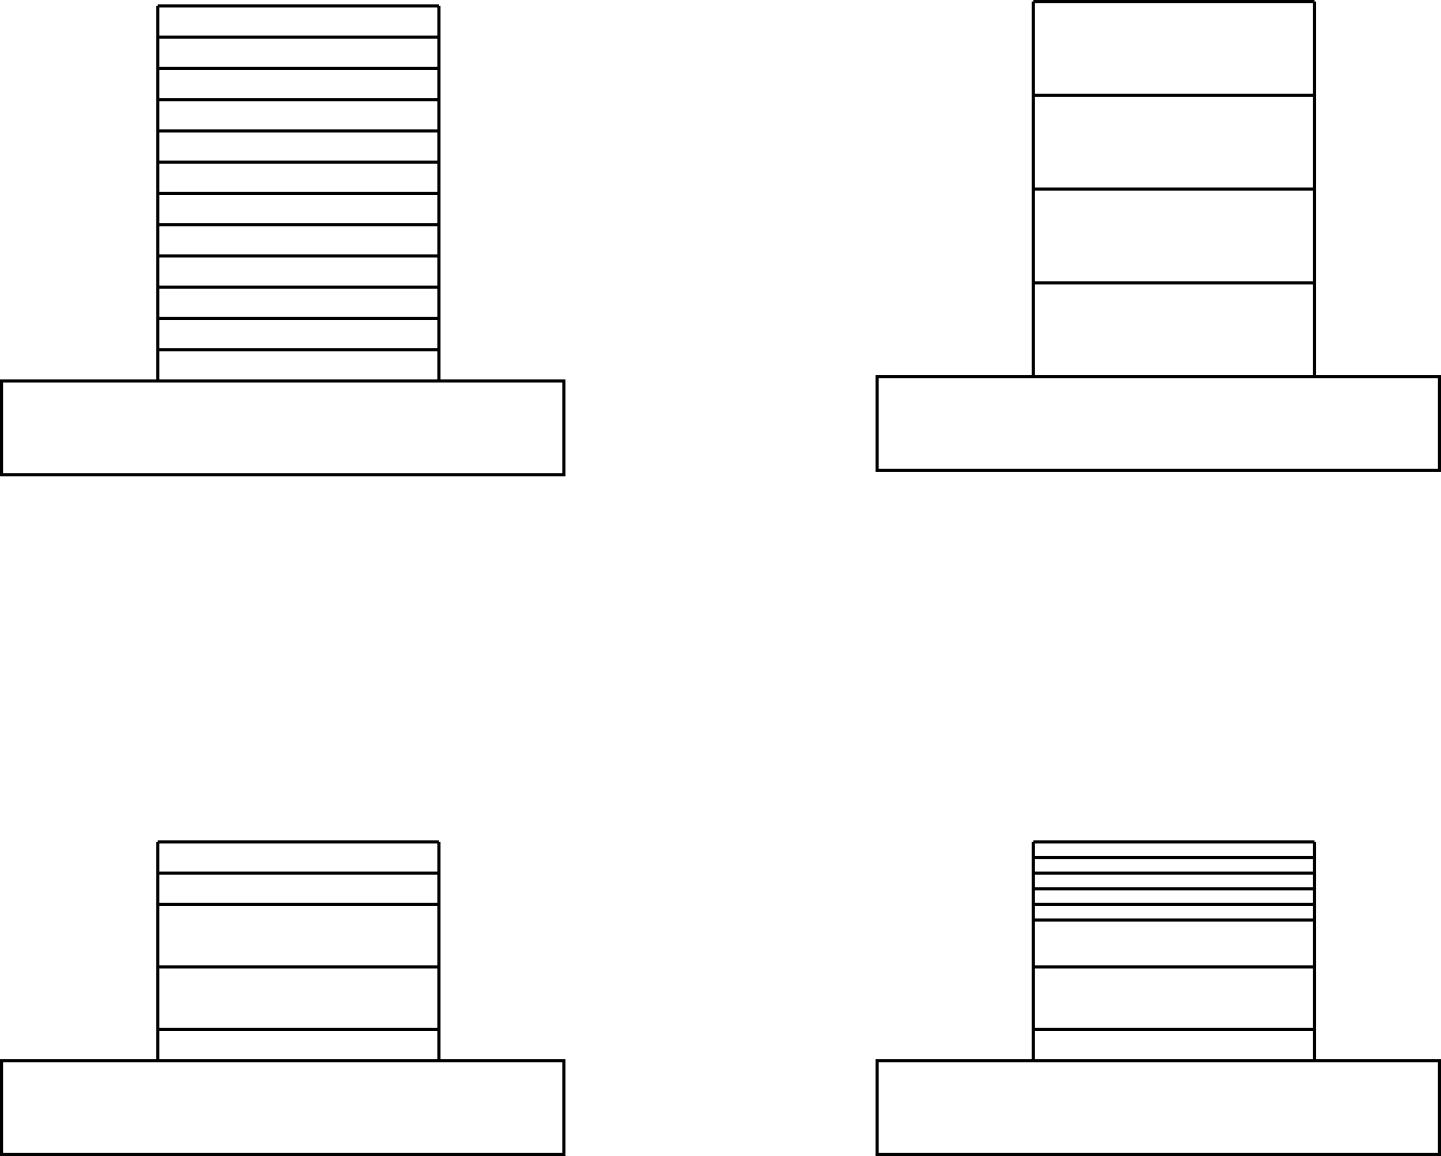
\includegraphics[width=6cm]{fig/2/20.png}
  \caption{左上为逐层的粗网格,右上为层合并的粗网格,左下是按照生死单元激活的粗网格,右下是对逐层部分根据单元进行加密。}
  \label{fig:2-1}
\end{figure}

另外一种首先对整个区域逐层进行细网格剖分,其次将一定层数进行合并,生成粗网格,这样获取两套一粗一细网格,然后根据带约束德洛内网格剖分的边界约束,可以将逐层部分和层合并部分根据生死单元激活进行组合,得到加密网格。

\begin{figure}[!htbp]
  \centering
  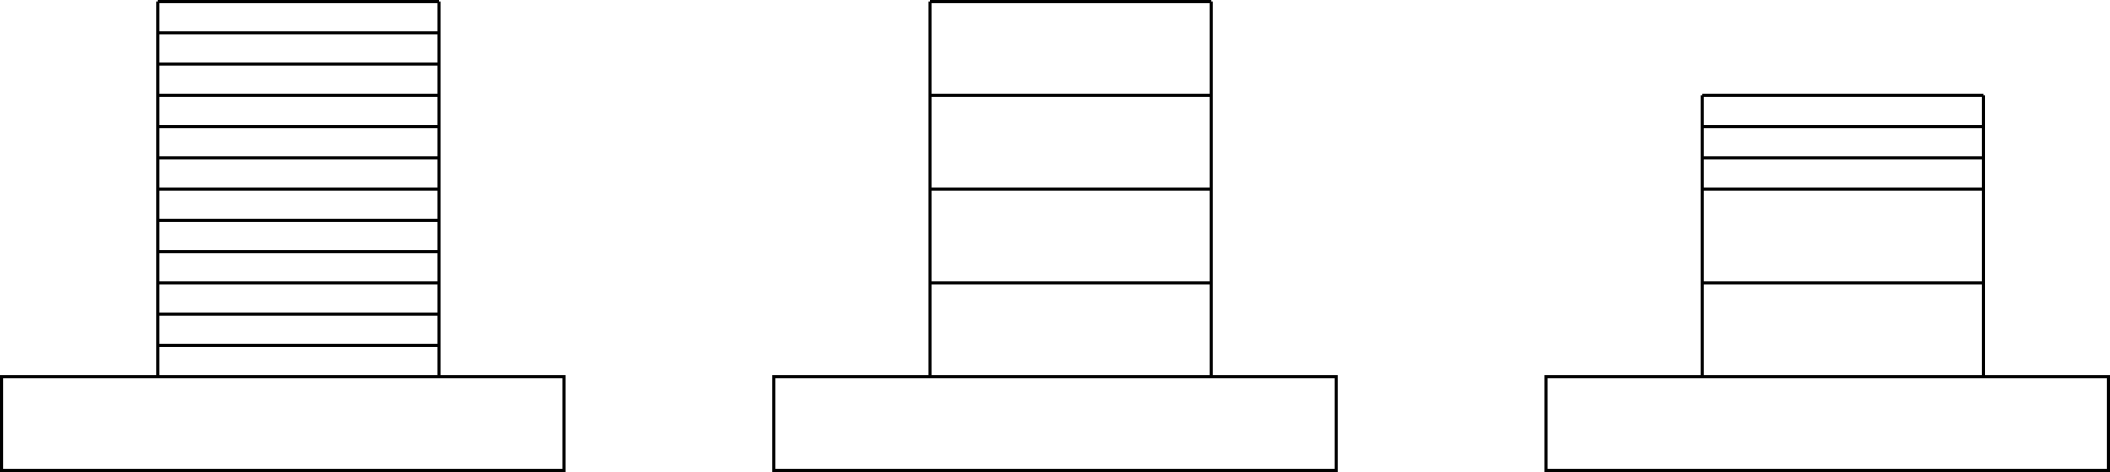
\includegraphics[width=10cm]{fig/2/21.png}
  \caption{左图为逐层的细网格,中图为层合并的粗网格,右图是按照生死单元激活的逐层部分加密网格。}
  \label{fig:2-1}
\end{figure}

\begin{figure}[!htbp]
  \centering
  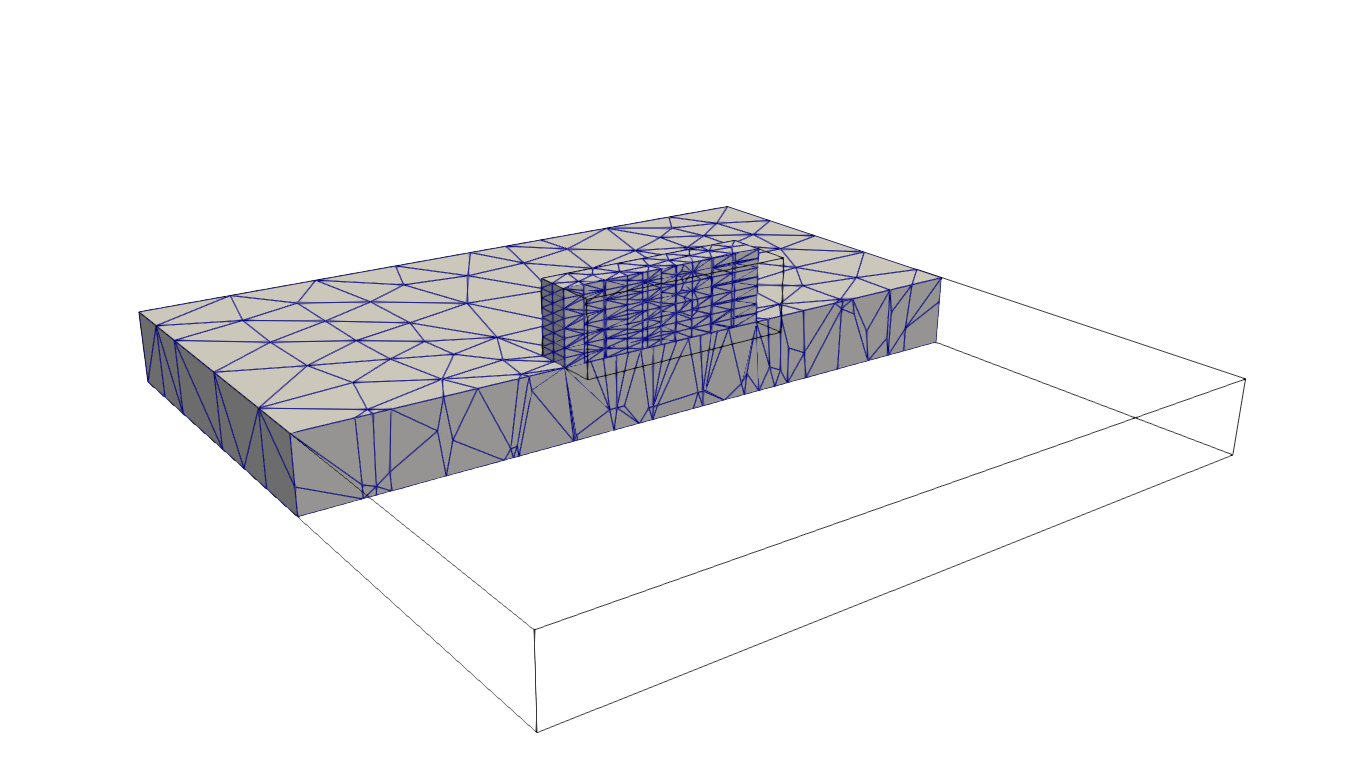
\includegraphics[height=6cm]{fig/2/22.png}
  \caption{加密}
  \label{fig:2-1}
\end{figure}

\begin{figure}[!htbp]
  \centering
  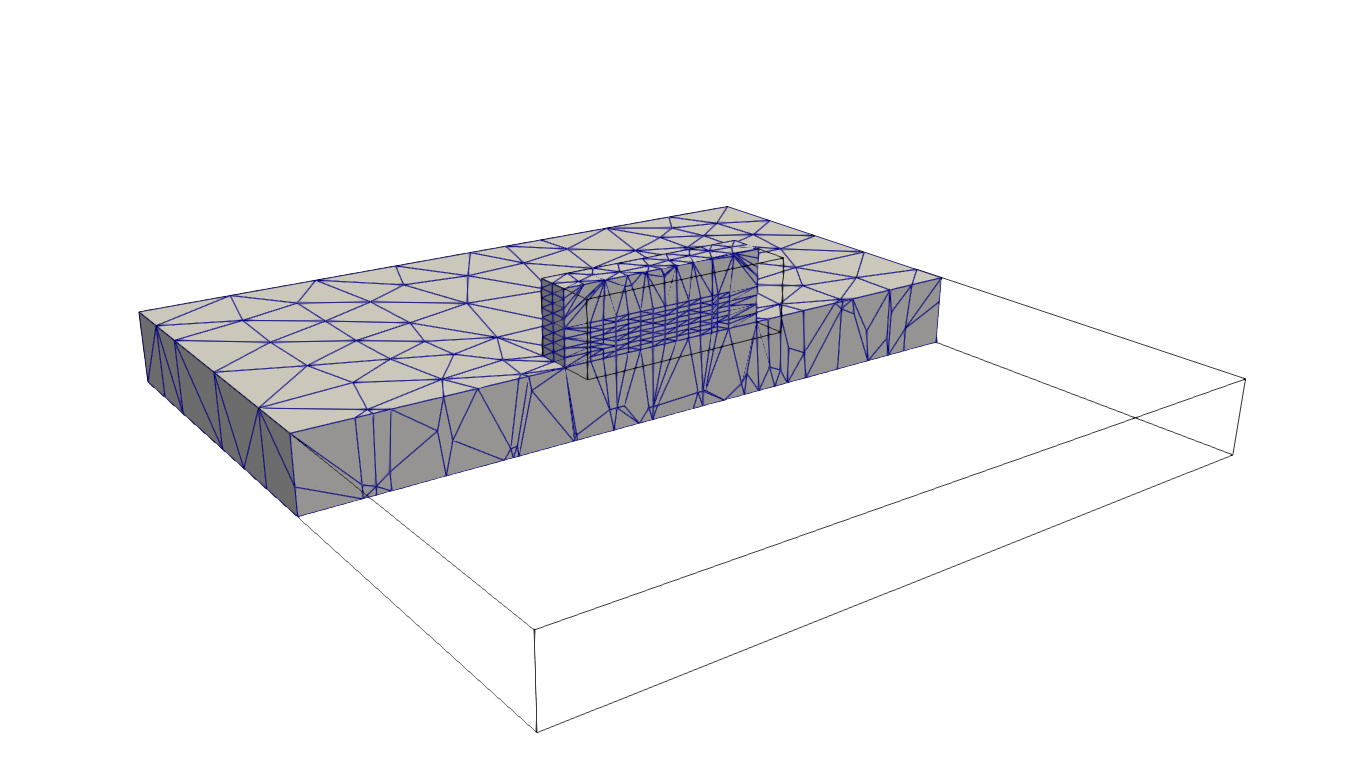
\includegraphics[height=6cm]{fig/2/23.png}
  \caption{放粗}
  \label{fig:2-1}
\end{figure}

\begin{figure}[!htbp]
  \centering
  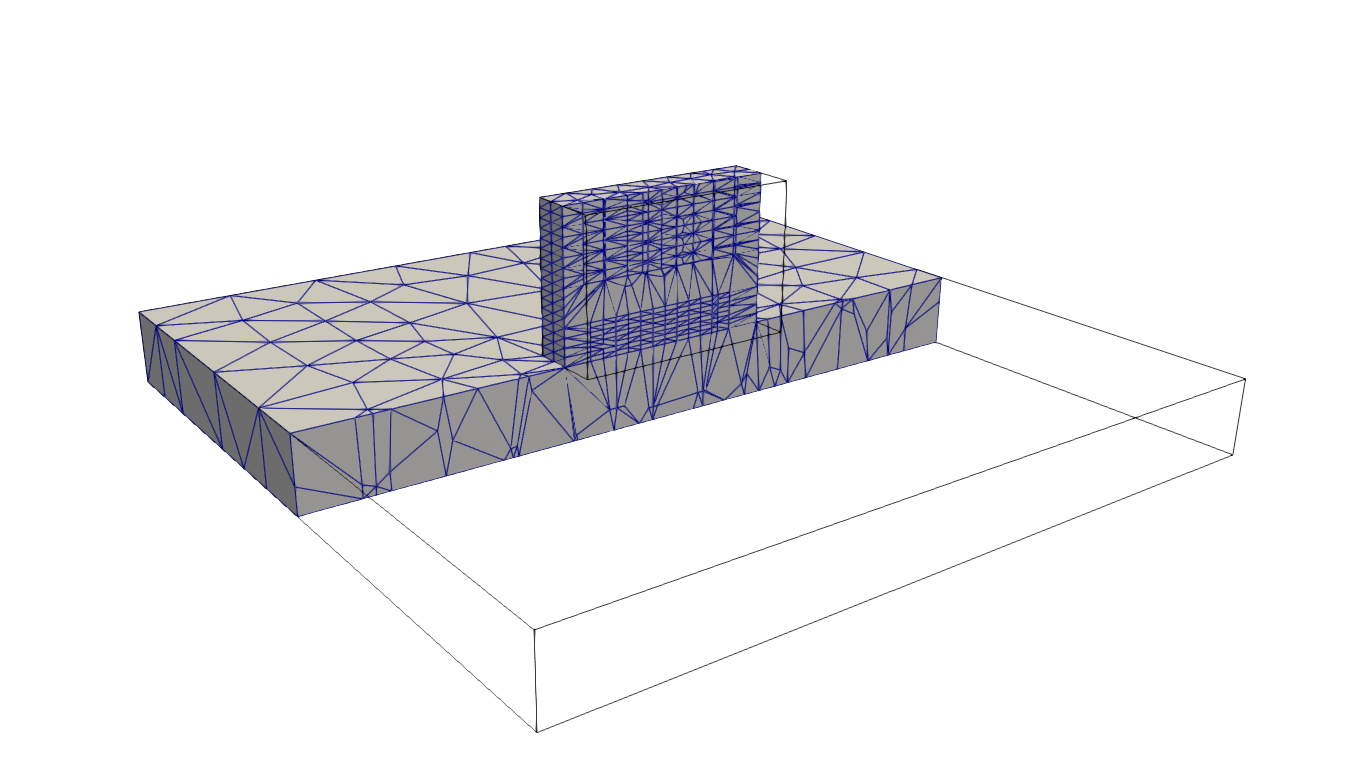
\includegraphics[height=6cm]{fig/2/24.png}
  \caption{加密}
  \label{fig:2-1}
\end{figure}

\begin{figure}[!htbp]
  \centering
  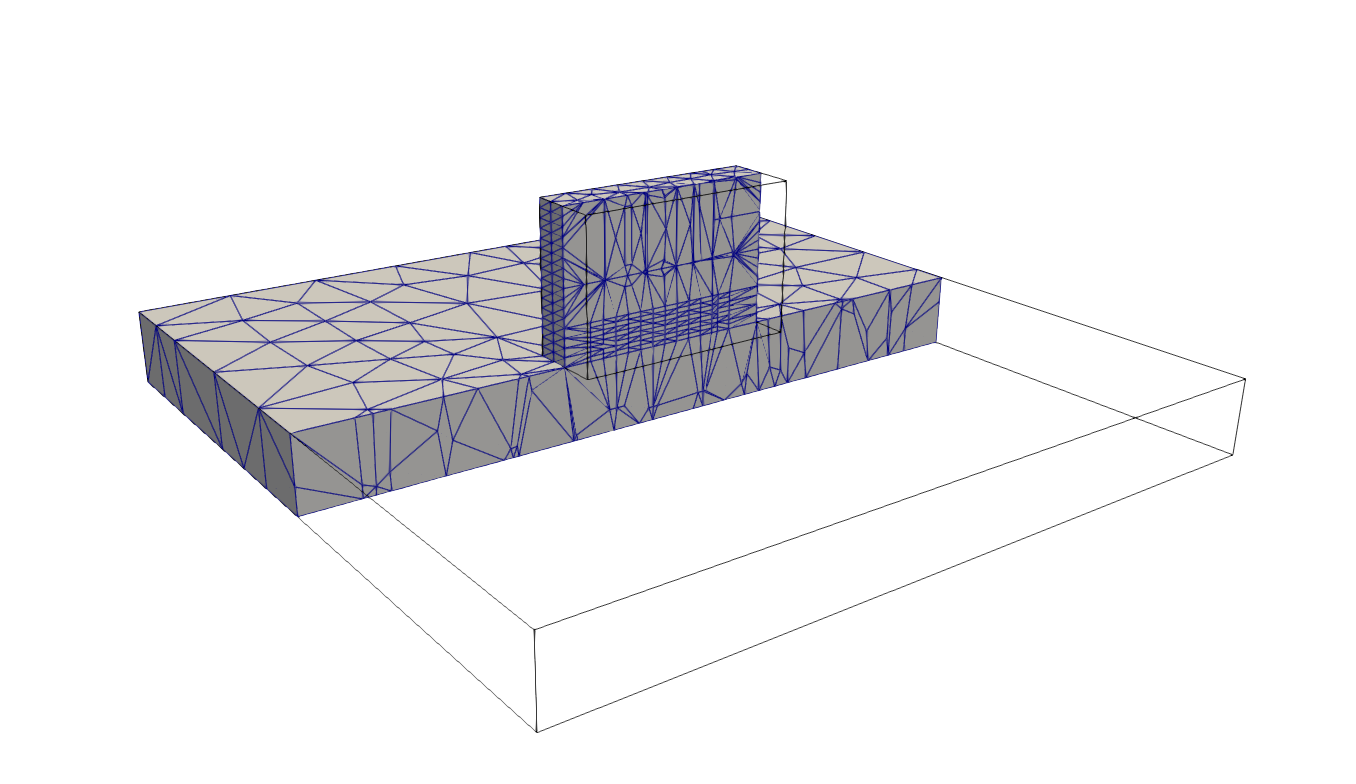
\includegraphics[height=6cm]{fig/2/25.png}
  \caption{放粗}
  \label{fig:2-1}
\end{figure}

\begin{figure}[!htbp]
  \centering
  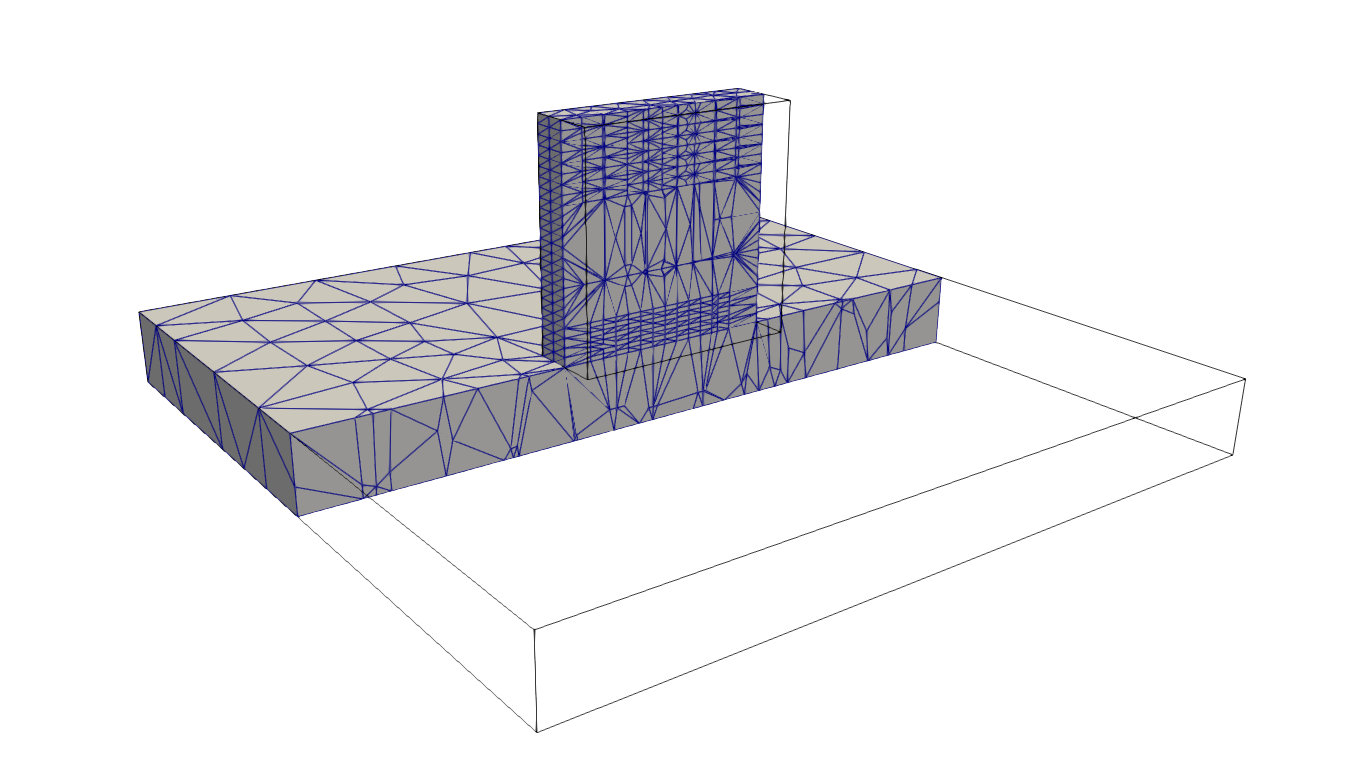
\includegraphics[height=6cm]{fig/2/26.png}
  \caption{加密}
  \label{fig:2-1}
\end{figure}

\begin{figure}[!htbp]
  \centering
  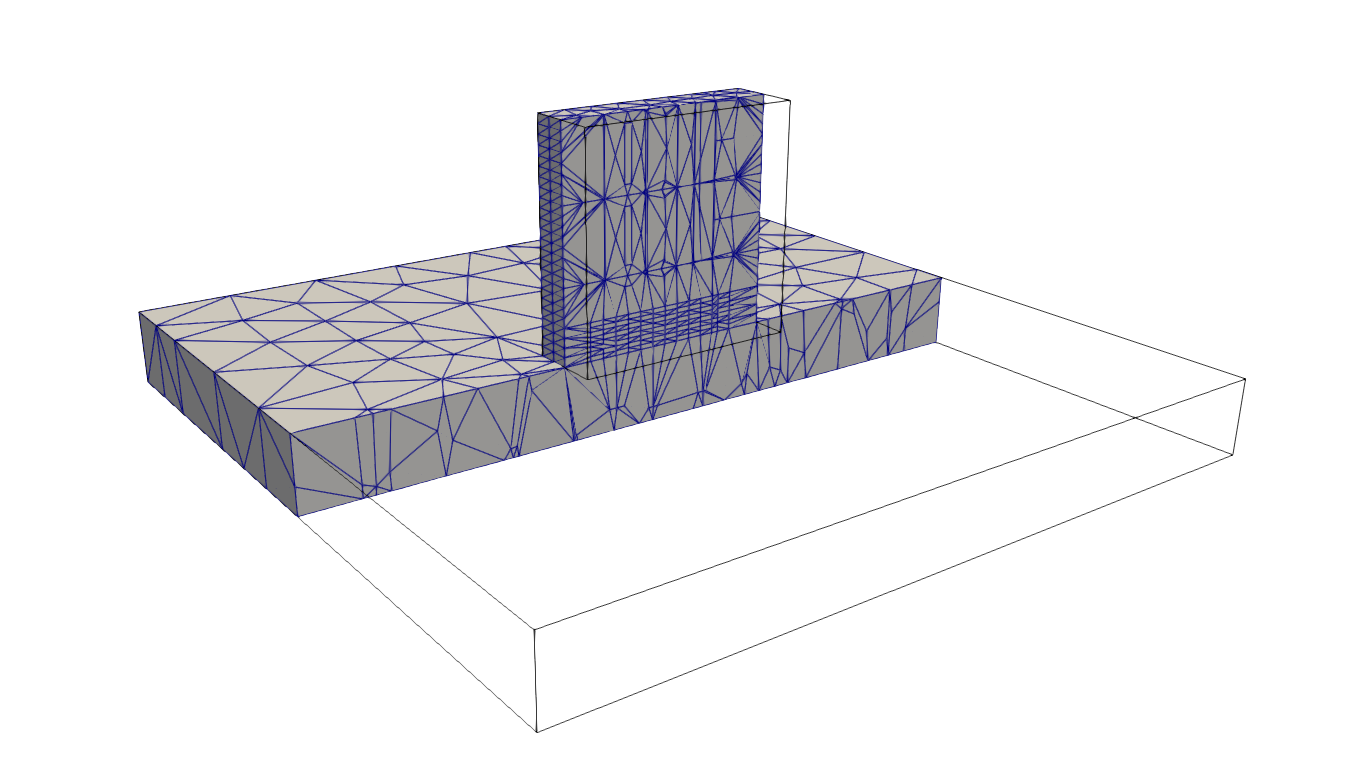
\includegraphics[height=6cm]{fig/2/27.png}
  \caption{放粗}
  \label{fig:2-1}
\end{figure}
